\documentclass[10pt,a4paper]{article}
\usepackage[utf8]{inputenc}
\usepackage{amsmath}
\usepackage{gensymb}
\usepackage{amsfonts}
\usepackage{siunitx}
\usepackage[european]{circuitikz}
\usepackage{geometry}
\newgeometry{tmargin=2cm, bmargin=2cm, lmargin=2cm, rmargin=2cm}
\usepackage{amssymb}
\usepackage{polski}
\usepackage{graphicx}
\author{\textbf{T. Fąs}}
\title{\textbf{DOŚWIADCZALNE SPRAWDZENIE DRUGIEJ ZASADY DYNAMIKI}}
\begin{document}
\maketitle


\begin{center}
\textbf{\subsection*{STRESZCZENIE}}
\end{center}
Celem doświadczenia było sprawdzenie, czy w warunkach eksperymentu spełniona jest druga zasada dynamiki Newtona. Udało się udowodnić, że przyśpieszenie jest wprost proporcjonalne do działającej siły oraz odwrotnie proporcjonalne do masy ciała. Dodatkowo, korzystając z wyznaczonej doświadczalnie masy układu, wyznaczono masę efektywną bloczka $m_{eff}=0,0598\pm0,0084$ kg.


\begin{center}
\textbf{\subsection*{WSTĘP}}
\end{center}
Zgodnie z drugą zasadą dynamiki Newtona, jeśli na ciało o masie $m$ działa siła $F$ lub siły o wypadkowej $F$, to ciało to porusza się z przyspieszeniem:
\begin{equation}
a=\dfrac{1}{m}F.
\end{equation}
Dla układu przedstawionego na Rysunku 1 zależność z Równania (1) przyjmuje postać:
\begin{equation}
a=\dfrac{mg}{M_{w}+M_{o}+m+I/R^2}=\dfrac{mg}{M},
\end{equation}
gdzie $I$ jest momentem bezwładności krążka, a $R$ jego promieniem.
Celem doświadczenia było sprawdzenie, czy przy stałej masie układu $M=M_{w}+M_{o}+m+I/R^2$ przyśpieszenie jest wprost proporcjonalne do siły oraz czy przy stałej sile $mg$ przyspieszenie jest odwrotnie proporcjonalne do masy. 


\begin{center}
\textbf{\subsection*{UKŁAD DOŚWIADCZALNY}}
\end{center}

\begin{figure}[h!]
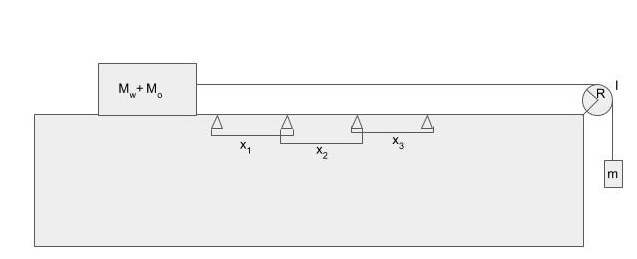
\includegraphics[width=15cm]{rap9rys1} 
\centering
\caption{Układ doświadczalny.}
\end{figure}


W doświadczeniu wykorzystano: wózek o masie $M_{w}$, 4 druty jako ciężarki o masie $m$, ciężarki o masach $M_{o}$, bloczek o promieniu zewnętrznym $R_{1}$ i wewnętrznym $R_{2}$ i o masie $m_{b}$, miarkę, wagę, nitkę oraz tor powietrzny wyposażony w fotokomórki. Układ był złożony tak, jak przedstawia to Rysunek 1, gdzie trójkąty symbolizują położenie fotokomórek.




\begin{center}
\textbf{\subsection*{WYNIKI POMIARÓW}}
\end{center}
W pierwszej kolejności zważono wózek oraz ciężarki i otrzymano wartości: $M_{w}=0,957$ kg, $M_{o1}=0,500$ kg, $M_{o2}=0,500$ kg, $M_{o3}=0,499$ kg,  $M_{o4}=0,250$ kg oraz $m=0,010$ kg dla każdego drutu. Za niepewność pomiaru przyjęto wartość $u_{m}=0,001$ kg. 

Następnie zmierzono szerokość fotokomórki $d=1,4$ cm i ustawiono je w odległościach $x_{1}=x_{2}=x_{3}=21,4$ cm. W ten sposób odległość między środkami fotokomórek wynosi 20 cm. Pomiarów dokonano przy pomocy miarki o działce pomiaru $\Delta_{x}=0,1$ cm. Działka pomiaru fotokomórki wynosi $\Delta_{t}=0,01$ s.

Przy takiej konfiguracji zmierzono trzykrotnie czasy przejazdu wózka między pierwszą fotokomórką, a każdą kolejną. W pierwszej części wózek był obciążony drutami i po każdych trzech pomiarach przekładano drut z wózka i doczepiano go do końcówki nitki. W ten sposób zwiększano siłę wymuszającą ruch, jednocześnie zachowując stałą masę układu. 

W drugiej części pomiarowej do końcówki nitki doczepiono cztery druty i nie zmieniano ich liczby przez cały czas trwania pomiaru. W ten sposób zapewniono stałość siły wymuszającej. Obciążenie wózka zmieniano wykorzystując ciężarki o masach 500 g i 250 g w różnych konfiguracjach. Obciążenie wózka było zmieniane po każdych trzech pomiarach czasu przejazdu. 

Po wykonaniu pomiarów przesunięto fotokomórki na nowe pozycje, tworząc tym samym nowe odległości i nowe punkty pomiarowe. Nowe odległości wynosiły: $x_{1}=26,4$ cm, $x_{2}=26,4$ cm, $x_{3}=18,4$ cm. Wszystkie wyniki zostały zebrane w Tabeli 1 i Tabeli 2 oraz Tabeli 3.

\begin{table}[h!]
\centering
\caption{Wyniki pomiarów: stała masa układu.}

\begin{tabular}{|c|c|c|c|c|c|c||c|c|c|c|c|c|}
\hline
\multicolumn{7}{|c|}{Jeden drucik ($m=0,01$ kg)}           & \multicolumn{6}{c|}{Dwa druciki ($m=0,02$ kg)}    \\ \hline
Odległość $s$ [m]  & 0,20 & 0,40 & 0,60 & 0,25 & 0,50 & 0,67 & 0,20   & 0,40   & 0,60   & 0,25  & 0,50  & 0,67 \\ \hline
Czas $t_{1}$ [s] & 1,36 & 2,17 & 2,83 & 1,58 & 2,48 & 2,98 & 0,95   & 1,52   & 1,98   & 1,10  & 1,74  & 2,09 \\ \hline
Czas $t_{2}$ [s] & 1,36 & 2,17 & 2,83 & 1,58 & 2,48 & 2,98 & 0,95   & 1,52   & 1,99   & 1,11  & 1,74  & 2,10 \\ \hline
Czas $t_{3}$ [s] & 1,36 & 2,17 & 2,84 & 1,57 & 2,48 & 2,98 & 0,95   & 1,52   & 1,99   & 1,11  & 1,74  & 2,10 \\ \hline
\multicolumn{7}{|c|}{Trzy druciki ($m=0,03$ kg)}           & \multicolumn{6}{c|}{Cztery druciki ($m=0,04$ kg)} \\ \hline
Czas $t_{1}$ [s] & 0,77 & 1,24 & 1,62 & 0,90 & 1,42 & 1,71 & 0,67   & 1,07   & 1,40   & 0,77  & 1,22  & 1,47 \\ \hline
Czas $t_{2}$ [s] & 0,77 & 1,24 & 1,62 & 0,90 & 1,42 & 1,70 & 0,67   & 1,07   & 1,40   & 0,78  & 1,22  & 1,47 \\ \hline
Czas $t_{3}$ [s] & 0,77 & 1,24 & 1,62 & 0,91 & 1,41 & 1,69 & 0,67   & 1,06   & 1,39   & 0,78  & 1,23  & 1,47 \\ \hline
\end{tabular}
\end{table}


\begin{table}[h!]
\centering
\caption{Wyniki pomiarów: stała siła}
\begin{tabular}{|c|c|c|c|c|c|c||c|c|c|c|c|c|}
\hline
\multicolumn{7}{|c|}{$M_{o}=0,25$ kg}                      & \multicolumn{6}{c|}{$M_{o}=0,5$ kg}     \\ \hline
Odległość [m]    & 0,20 & 0,40 & 0,60 & 0,25 & 0,50 & 0,67 & 0,20 & 0,40 & 0,60 & 0,25 & 0,50 & 0,67 \\ \hline
Czas $t_{1}$ [s] & 0,74 & 1,19 & 1,56 & 0,87 & 1,37 & 1,65 & 0,81 & 1,30 & 1,70 & 0,96 & 1,50 & 1,81 \\ \hline
Czas $t_{2}$ [s] & 0,74 & 1,19 & 1,56 & 0,87 & 1,37 & 1,65 & 0,81 & 1,30 & 1,70 & 0,95 & 1,50 & 1,80 \\ \hline
Czas $t_{3}$ [s] & 0,74 & 1,19 & 1,56 & 0,87 & 1,37 & 1,65 & 0,81 & 1,30 & 1,70 & 0,95 & 1,49 & 1,79 \\ \hline
\multicolumn{7}{|c|}{$M_{o}=0,75$ kg}                      & \multicolumn{6}{c|}{$M_{o}=1$ kg}       \\ \hline
Czas$t_{1}$ [s]  & 0,88 & 1,40 & 1,84 & 1,03 & 1,62 & 1,95 & 0,94 & 1,50 & 1,97 & 1,10 & 1,73 & 2,07 \\ \hline
Czas $t_{2}$ [s] & 0,89 & 1,40 & 1,84 & 1,03 & 1,62 & 1,95 & 0,94 & 1,50 & 1,97 & 1,10 & 1,73 & 2,08 \\ \hline
Czas $t_{3}$ [s] & 0,88 & 1,40 & 1,84 & 1,03 & 1,62 & 1,94 & 0,94 & 1,50 & 1,97 & 1,11 & 1,74 & 2,09 \\ \hline
\multicolumn{7}{|c|}{$M_{o}=1,25$ kg}                      & \multicolumn{6}{c|}{$M_{o}=1,5$ kg}     \\ \hline
Czas$t_{1}$ [s]  & 1,00 & 1,60 & 2,09 & 1,17 & 1,84 & 2,21 & 1,05 & 1,69 & 2,20 & 1,23 & 1,94 & 2,33 \\ \hline
Czas $t_{2}$ [s] & 1,00 & 1,60 & 2,09 & 1,17 & 1,84 & 2,21 & 1,05 & 1,69 & 2,20 & 1,24 & 1,94 & 2,33 \\ \hline
Czas $t_{3}$ [s] & 1,00 & 1,60 & 2,09 & 1,17 & 1,84 & 2,21 & 1,05 & 1,70 & 2,20 & 1,23 & 1,93 & 2,32 \\ \hline
\end{tabular}
\end{table}


\begin{table}[h!]
\centering
\caption{Stała siła: pomiar kontrolny}
\begin{tabular}{|c|c|c|c|c|c|c|}
\hline
\multicolumn{7}{|c|}{$M_{o}=0$ kg}                         \\ \hline
Odległość [m]    & 0,20 & 0,40 & 0,60 & 0,25 & 0,50 & 0,67 \\ \hline
Czas $t_{1}$ [s] & 0,67 & 1,07 & 1,40 & 0,78 & 1,23 & 1,47 \\ \hline
Czas $t_{2}$ [s] & 0,67 & 1,07 & 1,40 & 0,78 & 1,23 & 1,47 \\ \hline
Czas $t_{3}$ [s] & 0,67 & 1,07 & 1,40 & 0,78 & 1,23 & 1,47 \\ \hline
\end{tabular}
\end{table}



\begin{center}
\textbf{\subsection*{ANALIZA DANYCH}}
\end{center}
W pierwszej kolejności obliczono odległość $s$ między środkiem pierwszej fotokomórki i każdej kolejnej. Odległości te dane są wzorami:
\begin{eqnarray}
s_{1}=x_{1}-d \\
s_{2}=x_{1}+x_{2}-2d \\
s_{3}=x_{1}+x_{2}+x_{3}-3d
\end{eqnarray}

Otrzymano wartości takie jak w Tabeli 1. Niepewności tych wielkości można obliczyć, korzystając z metody propagacji małych błędów. Ogólny wzór przenoszenia niepewności w tej metodzie jest następujący:
 \begin{equation}
 u_{f}^2=\sum_{i=1}^n \left( \dfrac{\partial f}{\partial x_{i}}u_{i}\right)^2+\sum_{i=1, i\neq j}^n \left( \dfrac{\partial f}{\partial x_{i}}\dfrac{\partial f}{\partial x_{j}}c_{ij}\right),
 \end{equation}
 gdzie wielkość $f$ zależy od wielkości $x_{i}$ o niepewnościach $u_{i}$ i o ocenach kowariancji $c_{ij}$ \cite{tay2}. W rozpatrywanym przypadku kowariancja wynosi zero. Niepewność pomiaru odległości lub szerokości fotokomórki dana jest wzorem:
 \begin{equation}
 u_{x}=\dfrac{\Delta_{x}}{\sqrt{3}} \quad \cite{tay3}.
 \end{equation}
Łącząc Równanie (6) z Równaniem (5) i równaniem (7) otrzymano:
\begin{eqnarray}
u_{s1}=\dfrac{\sqrt{2}\Delta_{x}}{\sqrt{3}} \\
u_{s2}=\dfrac{2\Delta_{x}}{\sqrt{3}} \\
u_{s3}=\dfrac{\sqrt{6}\Delta_{x}}{\sqrt{3}}.
\end{eqnarray}

W przypadku analizy czasów przejazdu wyznaczono średnią dla każdego odcinka jak i niepewność tej średniej korzystając ze wzorów:
\begin{eqnarray}
\bar{t}=\sum_{i=1}^{n}\dfrac{t_{i}}{n} \\
f_{\bar{t}}^2=\sum_{i=1}^{n}\dfrac{\left(t_{i}-\bar{t}\right)^2}{n\left(n-1\right)}  \quad \cite{tay3}.
\end{eqnarray}
Przy czym na mocy równania (6) ostateczna niepewność pomiaru czasu dana jest wzorem;
\begin{equation}
u_{t}=\sqrt{f_{\bar{t}}^2+\dfrac{\Delta_{t}^2}{3}}.
\end{equation}

Wartości odległości, średniego czasu oraz ich niepewności znajdują się w Tabeli 4, Tabeli 5 i Tabeli 6.

\begin{table}[h!]
\centering
\caption{Analiza danych: stała masa układu.}
\begin{tabular}{|c|c|c|c|c|c|c|}
\hline
s [m]             & 0,200   & 0,400   & 0,600   & 0,250   & 0,500   & 0,670   \\ \hline
$u_{s}$ [m]       & 0,00082 & 0,00115 & 0,00141 & 0,00082 & 0,00115 & 0,00141 \\ \hline
\multicolumn{7}{|c|}{$m=0,01$ kg}                                             \\ \hline
$\bar{t}$ [s]     & 1,3600  & 2,1700  & 2,8333  & 1,5767  & 2,4800  & 2,9800  \\ \hline
$u_{\bar{t}}$ [s] & 0,0058  & 0,0058  & 0,0067  & 0,0067  & 0,0058  & 0,0058  \\ \hline
\multicolumn{7}{|c|}{$m=0,02$ kg}                                             \\ \hline
$\bar{t}$ [s]     & 0,9500  & 1,5200  & 1,9867  & 1,1067  & 1,7400  & 2,0967  \\ \hline
$u_{\bar{t}}$ [s] & 0,0058  & 0,0058  & 0,0067  & 0,0067  & 0,0058  & 0,0067  \\ \hline
\multicolumn{7}{|c|}{$m=0,03$ kg}                                             \\ \hline
$\bar{t}$ [s]     & 0,7700  & 1,2400  & 1,6200  & 0,9033  & 1,4167  & 1,7000  \\ \hline
$u_{\bar{t}}$ [s] & 0,0058  & 0,0058  & 0,0058  & 0,0067  & 0,0067  & 0,0082  \\ \hline
\multicolumn{7}{|c|}{$m=0,04$ kg}                                             \\ \hline
$\bar{t}$ [s]     & 0,6700  & 1,0667  & 1,3967  & 0,7767  & 1,2233  & 1,4700  \\ \hline
$u_{\bar{t}}$ [s] & 0,0058  & 0,0067  & 0,0067  & 0,0067  & 0,0067  & 0,0058  \\ \hline
\end{tabular}
\end{table}




\begin{table}[h!]
\caption{Analiza danych: stała siła.}
\setlength\tabcolsep{4 pt}
\begin{minipage}{0.5\textwidth}
\centering

\begin{tabular}{|c|c|c|c|c|c|c||c|c|c|c|c|c|}
\hline
s [m]             & 0,20000  & 0,4000   & 0,6000   & 0,2500   & 0,5000   & 0,6700   & 0,20000 & 0,4000 & 0,6000 & 0,2500 & 0,5000 & 0,6700 \\ \hline
$u_{s}$ [m]       & 0,00082 & 0,00115 & 0,00141 & 0,00082 & 0,00115 & 0,00141 & 0,00082 & 0,0012 & 0,0014 & 0,0008 & 0,0012 & 0,0014 \\ \hline
\multicolumn{7}{|c|}{$M_{o}=0,25$ kg}                                         & \multicolumn{6}{c|}{$M_{o}=0,5$ kg}                  \\ \hline
$\bar{t}$ [s]     & 0,7400  & 1,1900  & 1,5600  & 0,8700  & 1,3700  & 1,6500  & 0,8100  & 1,3000 & 1,7000 & 0,9533 & 1,4967 & 1,8000 \\ \hline
$u_{\bar{t}}$ [s] & 0,0058  & 0,0058  & 0,0058  & 0,0058  & 0,0058  & 0,0058  & 0,0058  & 0,0058 & 0,0058 & 0,0442 & 0,0442 & 0,0580 \\ \hline
\multicolumn{7}{|c|}{$M_{o}=0,75$ kg}                                         & \multicolumn{6}{c|}{$M_{o}=1$ kg}                    \\ \hline
$\bar{t}$ [s]     & 0,8833  & 1,4000  & 1,8400  & 1,0300  & 1,6200  & 1,9467  & 0,9400  & 1,5000 & 1,9700 & 1,1033 & 1,7333 & 2,0800 \\ \hline
$u_{\bar{t}}$ [s] & 0,0442  & 0,0058  & 0,0058  & 0,0058  & 0,0058  & 0,0442  & 0,0058  & 0,0058 & 0,0058 & 0,0442 & 0,0442 & 0,0580 \\ \hline
\multicolumn{7}{|c|}{$M_{o}=1,25$ kg}                                         & \multicolumn{6}{c|}{$M_{o}=1,5$ kg}                  \\ \hline
$\bar{t}$ [s]     & 1,0000  & 1,6000  & 2,0900  & 1,1700  & 1,8400  & 2,2100  & 1,0500  & 1,6933 & 2,2000 & 1,2333 & 1,9367 & 2,3267 \\ \hline
$u_{\bar{t}}$ [s] & 0,0058  & 0,0058  & 0,0058  & 0,0058  & 0,0058  & 0,0058  & 0,0058  & 0,0442 & 0,0058 & 0,0442 & 0,0442 & 0,0442 \\ \hline
\end{tabular}
\end{minipage}
\end{table}


\begin{table}[h!]
\centering
\caption{Stała siła: pomiar kontrolny.}
\begin{tabular}{|c|c|c|c|c|c|c|}
\hline
s [m]             & 0,200   & 0,400   & 0,600   & 0,250   & 0,500   & 0,670   \\ \hline
$u_{s}$ [m]       & 0,00082 & 0,00115 & 0,00141 & 0,00082 & 0,00115 & 0,00141 \\ \hline
\multicolumn{7}{|c|}{$M_{o}=0$ kg}                                            \\ \hline
$\bar{t}$ [s]     & 0,6700  & 1,0700  & 1,4000  & 0,7800  & 1,2300  & 1,4700  \\ \hline
$u_{\bar{t}}$ [s] & 0,0058  & 0,0058  & 0,0058  & 0,0058  & 0,0058  & 0,0058  \\ \hline
\end{tabular}
\end{table}

W dalszej części analizy zastąpiono oznaczenie $\bar{t}$ zwykłym $t$ ze względu na prostotę i estetykę.

Zależność $s(t)$ jest klasycznym przykładem prostoliniowego ruchu z przyśpieszeniem, który wyraża się wzorem:
\begin{equation}
r(t)=r_{0}+v_{0}t+\dfrac{1}{2}at^2,
\end{equation}
gdzie $r_{0}$ jest położeniem początkowym, a $v_{0}$ jest prędkością początkową. Zależność tę można sprowadzić do postaci liniowej dzieląc obie strony przez $t$:
\begin{equation}
\dfrac{r-r_{0}}{t}=v_{0}+\dfrac{1}{2}at
\end{equation}
Dodatkowo w rozpatrywanym przypadku $r-r_{0}=s$, co dodatkowo upraszcza zależność. 
Oznaczając $s/t=w$ można tę zależność zapisać jako:
\begin{equation}
w=At+B,
\end{equation}
gdzie $a=0,5\cdot a$, $B=v_{0}$. Aby znaleźć wartości przyśpieszeń, należy do punktów z Tabeli 5 dopasować prostą według Równania (15) i Równania (16). W tym celu posłużono się metodą najmniejszych kwadratów. Polega ona na minimalizacji wielkości, która w tym przypadku dana jest wzorem:
\begin{equation}
R\left(A, B \right)=\sum_{i=1}^{6}\left(\dfrac{w_{i}-At-B}{u_{w_{i}}}\right)^2 \quad \cite{tay1}
\end{equation}
Niepewności $w_{i}$ otrzymano, korzystając z Równania (6):
\begin{equation}
u_{w_{i}}=w_{i}\sqrt{\dfrac{u_{t_{i}}^2}{t_{i}^2}+\dfrac{u_{s_{i}}^2}{s_{i}^2}}
\end{equation}
Ostateczne wartości parametrów wraz z ich niepewnościami podano w Tabeli 7. dodatkowo podano też wartości przyśpieszeń $a$ wraz z niepewnościami.

\begin{table}[h!]
\centering
\caption{Dopasowywanie prostej: stała masa układu.}

\begin{tabular}{|c|c|c|c|c|}
\hline
$m$ [kg]          & 0,01    & 0,02   & 0,03   & 0,04   \\ \hline
$A$ [m/s$^2$]     & 0,04632 & 0,0925 & 0,1382 & 0,1896 \\ \hline
$u_{A}$ [m/s$^2$] & 0,00052 & 0,0013 & 0,0024 & 0,0035 \\ \hline
$B$ [m/s]         & 0,08471 & 0,1233 & 0,1527 & 0,1730 \\ \hline
$u_{B}$ [m/s]     & 0,00126 & 0,0023 & 0,0033 & 0,0042 \\ \hline
$a$ [m/s$^2$]     & 0,0926  & 0,1850 & 0,2763 & 0,3792 \\ \hline
$u_{a}$ [m/s$^2$] & 0,0010  & 0,0027 & 0,0048 & 0,0070 \\ \hline
\end{tabular}
\end{table}

W ten sposób otrzymano zestaw punktów pozwalających na sprawdzenie zależności opisanej przez Równanie (2). Aby dopasować dane z Tabeli 7 do Równania (2) ponownie zastosowano metodę najmniejszych kwadratów oraz Równanie (17) dla $B=0$. Przyjęto, że $g=9,81$ m/s$^2$ jest wartością znaną dokładnie. Wyniki tej analizy przedstawiono w Tabeli 8. Krzywą najlepszego dopasowania, wraz ze słupkami niepewności przedstawiono na Rysunku 2.

\begin{table}[h!]
\centering
\caption{Regresja liniowa: stała masa układu.}
\begin{tabular}{|c|c|c|c|c|}
\hline
$m$ [kg]          & 0,01    & 0,02   & 0,03   & 0,04   \\ \hline
$mg$ [N]          & 0,04632 & 0,0925 & 0,1382 & 0,1896 \\ \hline
$a$ [m/s$^2$]     & 0,0926  & 0,1850 & 0,2763 & 0,3792 \\ \hline
$u_{a}$ [m/s$^2$] & 0,0010  & 0,0027 & 0,0048 & 0,0070 \\ \hline
\multicolumn{5}{|c|}{$1/M_{d}=0,9462\pm 0,0069$ 1/kg}      \\ \hline
\end{tabular}
\end{table}


\begin{figure}[h!]
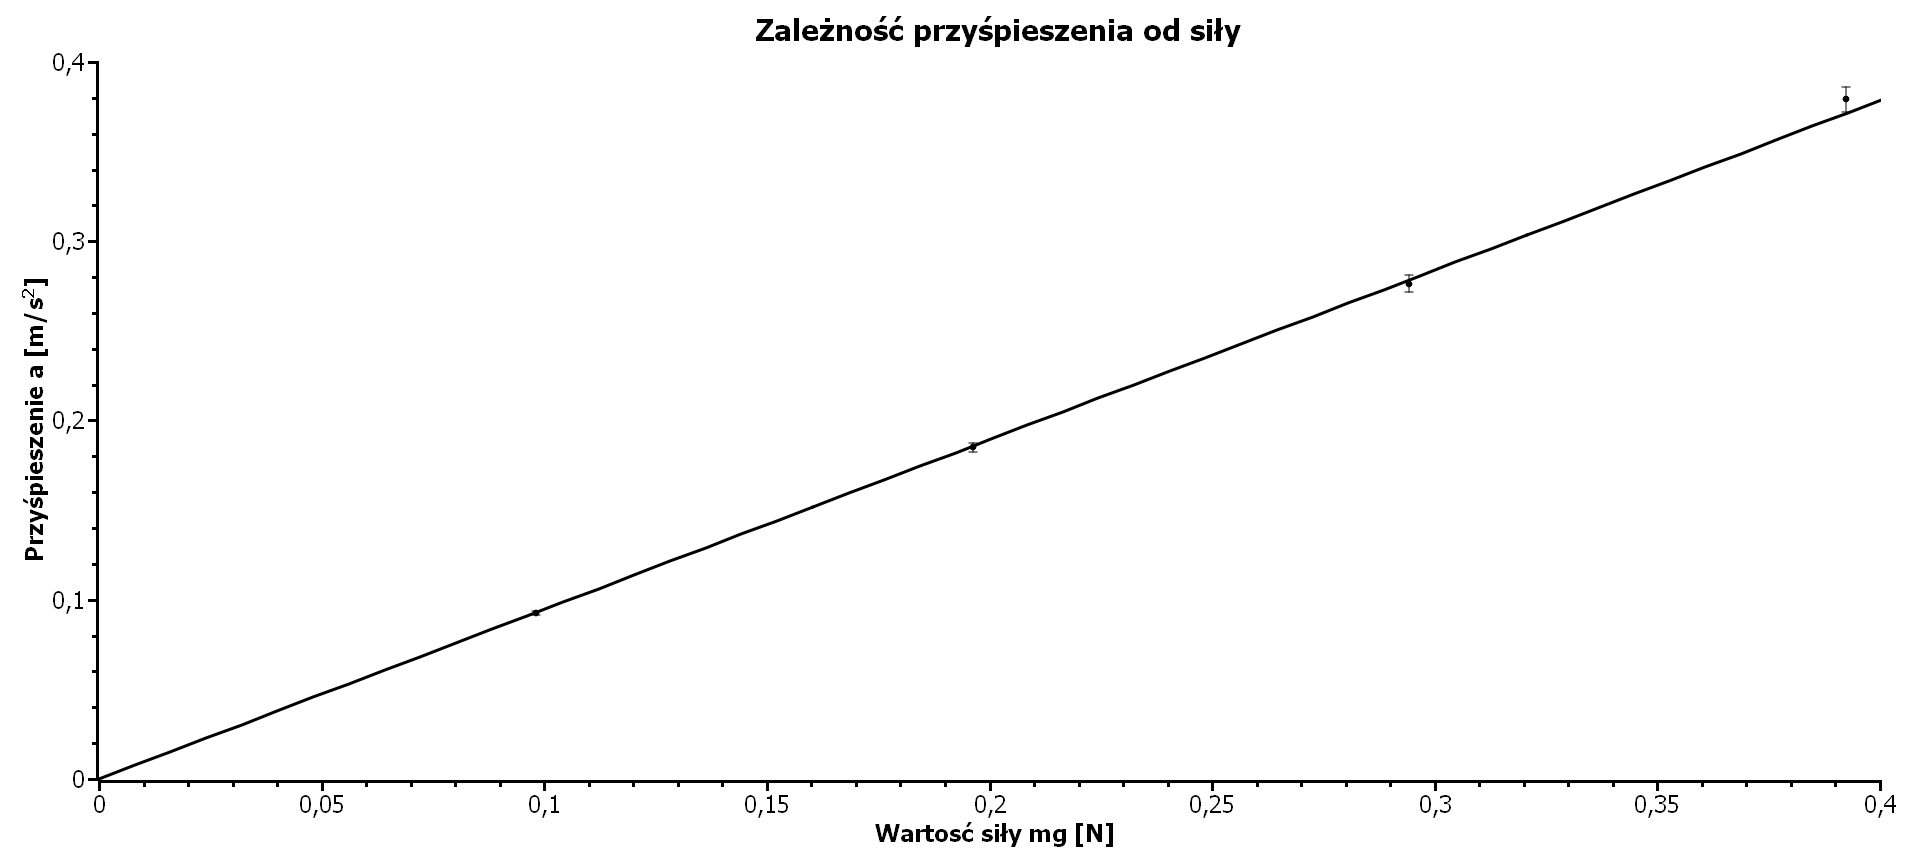
\includegraphics[width=15cm]{rap9rys2} 
\centering
\caption{Krzywa najlepszego dopasowania.}
\end{figure}

Aby zyskać pewność, co do poprawnego dopasowania krzywej, przeprowadzono test $\chi^2$. Test ten pozwoli też określić, czy dane są w zgodności z drugą zasadą dynamiki.

W rozpatrywanym przypadku wartość $\chi^2$ dana jest wzorem:
\begin{equation}
\chi^2=\sum_{i=1}^{4}\left(\dfrac{a_{i}-\dfrac{1}{M_{d}}F_{i}}{u_{a_{i}}}\right)^2
\end{equation}
Za prawdopodobieństwo popełnienia błędu pierwszego rodzaju przyjęto $p=0,005$ . Przy 4-1=3 stopniach swobody wartość krytyczna $\chi_{0}^2=12,84$ Wartość obliczona wynosi $\chi^2=1,57$. Wartość ta jest mniejsza od wartości krytycznej, czyli dane otrzymane w doświadczeniu nie są sprzeczne z drugą zasadą dynamiki Newtona.  

Współczynnik $M_{d}$ jest masą układu wyznaczoną doświadczalnie. Można porównać ją z wartością otrzymaną w bezpośrednich pomiarach mas wózka i drutów. Wiadomo, że masa krążka wynosiła $m_{b}=36$ g, a jego promienie, zewnętrzny i wewnętrzny wynosiły kolejno: $R_{1}=96$ mm i $R_{2}=8$ mm. Bezwładność krążka wynosiła $I=\dfrac{1}{2}m_{b}(R_{1}^2+R_{2}^2)$. Oznaczmy $I/mR_{1}^2=m_{eff}$. Wtedy $M=M_{w}+4m+m_{eff}=1,0568$ kg. Niepewność tej wielkości obliczono, korzystając z Równania (6). Otrzymano $u_{M}=0,0065$ kg. W analizie danych założono, że wielkość $m_{eff}$ jest znana dokładnie. Aby porównać, czy $M$ jest zgodne z wartością $M_{d}$ przeprowadzono test 3$\sigma$. Polega on na sprawdzeniu, czy wielkość $|M-M_{d}|$ jest mniejsza od trzykrotności niepewności tej różnicy. Otrzymano wartości: ($|M-M_{d}|=(0,0477>3*0,077)$ kg. Jak widać, współczynniki te nie są ze sobą zgodne. Mimo to postanowiono założyć, że $M_{d}=M_{w}+4m+m_{eff}$ aby obliczyć eksperymentalną wartość masy efektywnej $m_{deff}$. Niepewność tej wielkości obliczono, korzystając z Równania (6). Otrzymano :$m_{deff}=0,0598\pm0,0084$ kg. Porównując tę wartość z wartością $m_{eff}$ i przeprowadzając test 3$\sigma$ otrzymano zgodność wyników. Zgodność wyników wynika z dużej niepewności, jaką obarczona jest wielkość $m_{deff}$.


Szukanie przyśpieszeń dla stałej siły wymuszającej wyglądało podobnie, jak w przypadku stałej masy układu. Wyniki analizy dla wartości z Tabeli 5 i Tabeli 6 przedstawiono w Tabeli 9. 

\begin{table}[h!]
\centering
\caption{Analiza danych: stała siła.}
\begin{tabular}{|c|c|c|c|c|c|c|c|}
\hline
$M_{o}$ [kg]      & 0      & 0,25   & 0,50   & 0,75   & 1,00   & 1,25   & 1,50   \\ \hline
$a$ [m/s$^2$]     & 0,3772 & 0,2934 & 0,2379 & 0,2067 & 0,1775 & 0,1671 & 0,1436 \\ \hline
$u_{a}$ [m/s$^2$] & 0,0066 & 0,0049 & 0,0055 & 0,0047 & 0,0037 & 0,0022 & 0,0028 \\ \hline
\end{tabular}
\end{table}

W przypadku stałej siły wymuszającej Równanie (2) można przekształcić do postaci:
\begin{equation}
\dfrac{g}{a_{i}}=\dfrac{1}{4m}M_{i}+\left(1+\dfrac{I}{4mR_{1}^2}\right),
\end{equation}
gdzie $M_{i}$ to masa układu przy i-tym pomiarze.

W ten sposób otrzymano zależność liniową $\eta=\alpha M_{i}+\beta$. Do takiej zależności można dostosować prostą przy pomocy metody najmniejszych kwadratów. Stosując Równanie (17) oraz Równanie (6) względem Równania (20) otrzymano wartości przedstawione w Tabeli 10.

\begin{table}[h!]
\centering
\caption{Regresja liniowa: stała siła.}
\begin{tabular}{|c|c|c|c|c|c|c|c|}
\hline
$M_{i}$ [kg]      & 0,9970  & 1,2470  & 1,4970  & 1,7470   & 1,9970  & 2,2470  & 2,4970  \\ \hline
$a_{i}$ [m/s$^2$] & 0,3780  & 0,2955  & 0,2496  & 0,2172   & 0,1879  & 0,1678  & 0,1502  \\ \hline
$u_{a}$ [m/s$^2$] & 0,0537  & 0,0428  & 0,0400  & 0,0338   & 0,0293  & 0,0238  & 0,0229  \\ \hline
$g/a_{i}$         & 25,9511 & 33,1986 & 39,3085 & 45,1585  & 52,2099 & 58,4574 & 65,2923 \\ \hline
$u_{gai}$         & 3,6888  & 4,8080  & 6,3008  & 7,0204   & 8,1370  & 8,3026  & 9,9342  \\ \hline
\multicolumn{4}{|c|}{$\alpha=25,92\pm0,35$ 1/kg}  & \multicolumn{4}{c|}{$\beta=0,38\pm0,63$} \\ \hline
\end{tabular}
\end{table}

Krzywą na podstawie tych danych przedstawiono na Rysunku 3.

\begin{figure}[h!]
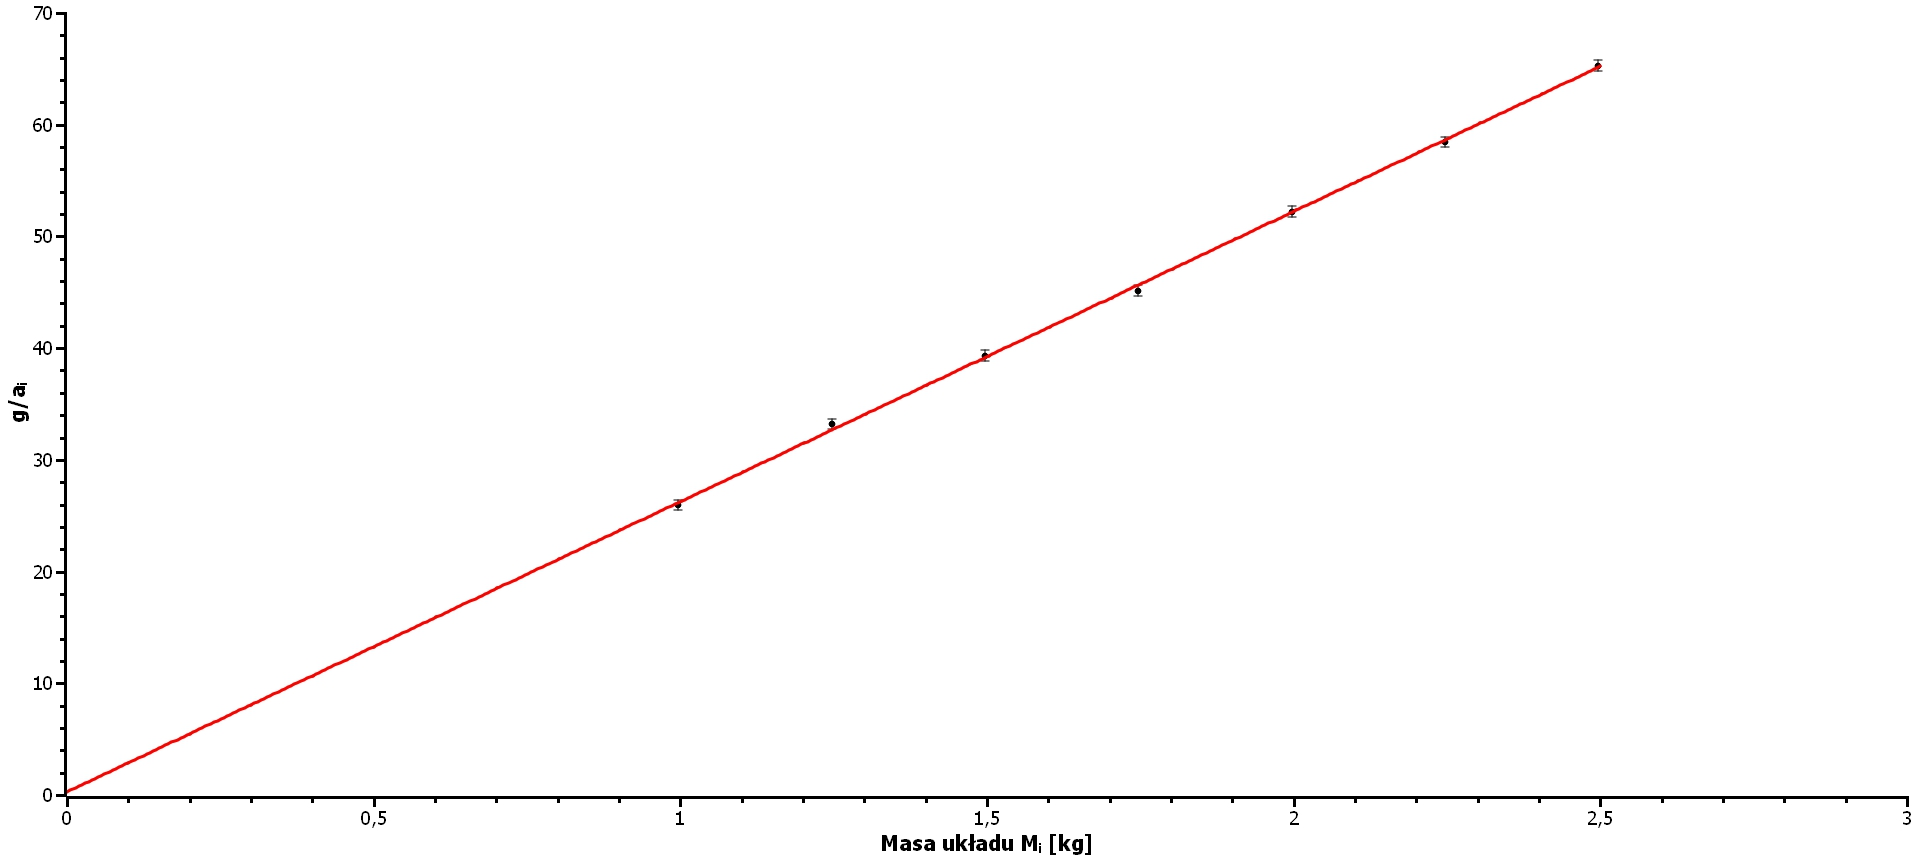
\includegraphics[width=13cm]{rap9rys3} 
\centering
\caption{Krzywa najlepszego dopasowania.}
\end{figure}


Obliczono wartość $\chi^2=0,31$, przy czym wartość krytyczna dla 7-2=5 punktów swobody wynosi $\chi_{0}^2=16,75$. $\chi^2<\chi_{0}^2$ więc dane nie są sprzeczne z drugą zasadą dynamiki Newtona. Warto jeszcze porównać otrzymane współczynniki z ich wartościami teoretycznymi. 

Wartość $1/4m=25$ 1/kg dla drucików o $m=0,01\pm0,001$ kg. Przeprowadzając test 3$\sigma$ dla tej wartości i wartości $\alpha$ uzyskano zgodność wyników. Zaniechano przeprowadzenie testu dla wartości $\beta$, gdyż jej wartość jest mniejsza od niepewności z nią związaną oraz dlatego, iż aktualna wartość $\beta$ sugeruje ujemną wartość bezwładności krążka.

\begin{center}
\textbf{\subsection*{DYSKUSJA WYNIKÓW I WNIOSKI}}
\end{center} 
W obu przypadka uzyskano zgodność danych z drugą zasadą dynamiki. Jednak niepokojącym jest fakt, iż nie zawsze udało się uzyskać zgodność wyznaczonych współczynników z ich przewidywaniami teoretycznymi. Prawdopodobnie wynika to z propagacji błędów przez wszystkie etapy analizy. Jednak w ogólności, zważywszy na niskie wartości $\chi^2$, można stwierdzić, iż w warunkach eksperymentu druga zasada dynamiki jest spełniona.



\begin{center}
\begin{thebibliography}{9}

 \bibitem{tay2}
 J. R. Taylor,
 \emph{Wstęp do analizy błędu pomiarowego},
 PWN, Warszawa, 1995, s. 197.
 
   \bibitem{tay3}
 J. R. Taylor,
 \emph{Wstęp do analizy błędu pomiarowego},
 PWN, Warszawa, 1995, s. 101.
 
 \bibitem{tay1}
 J. R. Taylor,
 \emph{Wstęp do analizy błędu pomiarowego},
 PWN, Warszawa, 1995, s. 175.
 
\end{thebibliography}

\end{center}


\end{document}